\documentclass{beamer}
\usepackage[italian]{isodate}  		% formato delle date in italiano
\usepackage[italian]{babel}
\usepackage{booktabs}				% tabelle di qualità superiore
\usepackage{amsmath}				% pacchetto matematica
\usepackage{pifont}					% pacchetto con elenchi carini
\usepackage{caption}				% pacchetto per gestiore \caption
\usepackage{ragged2e}				% pacchetto per \justifying

\newcommand{\longline}{\noindent\rule{\textwidth}{0.4pt}}
\newcommand{\dquotes}[1]{``#1''}

% Informations:
\usetheme{Marburg}
\usefonttheme{serif}
\setbeamertemplate{itemize item}[circle]
\setbeamertemplate{footline}[frame number]
\setbeamertemplate{navigation symbols}{}%remove navigation symbols

\title{Tesina su FaaS (Function-as-a-Service)}
\author{VR443470 - Valentini Andrea}
\institute{Università degli studi di Verona}
\date{\printdayoff\today}
\titlegraphic{
	
\includegraphics[width=.6\textwidth]{img/faas-1.jpg}
}
\apptocmd{\frame}{}{\justifying}{} % Allow optional arguments after frame.


\begin{document}
	
	% Title
	\begin{frame}
		\titlepage
	\end{frame}
	
	% Index
	\begin{frame}
		\frametitle{Contenuti}
		\tableofcontents
	\end{frame}
	
	\section{Introduzione}
	\begin{frame}
		\frametitle{Introduzione}
		\framesubtitle{La crescita esponenziale dei servizi cloud}
		Con l'avanzare della tecnologia, il \emph{cloud computing} è diventato un servizio sempre più richiesto. La sua crescita è stata influenzata anche dalla pandemia mondiale COVID-19.
		\begin{figure}
			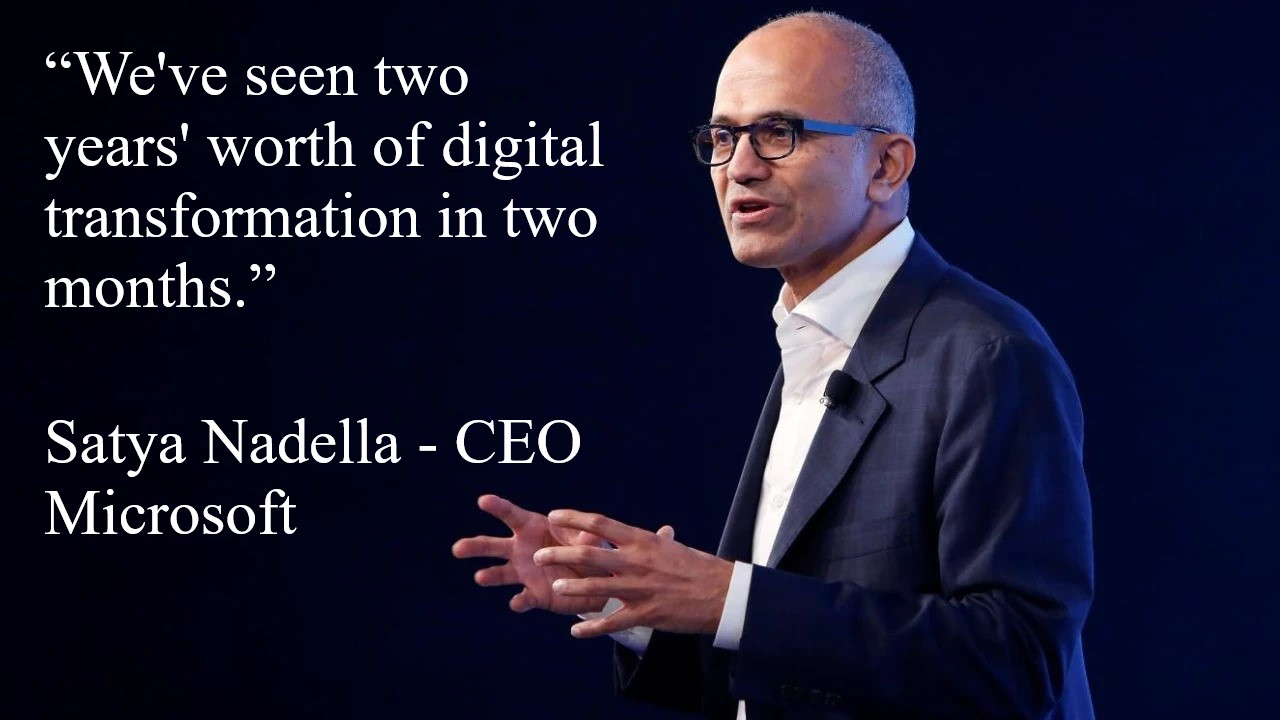
\includegraphics[width=.7\textwidth]{img/satya-nadella-microsoft-mod.jpg}
			\caption*{\dquotes{\emph{Abbiamo assistito a due anni di trasformazione digitale in due mesi}}\newline
			$\sim$ Satya Nadella, CEO Microsoft\footnote{\href{https://www.microsoft.com/en-us/microsoft-365/blog/2020/04/30/2-years-digital-transformation-2-months/}{Link dell'articolo}}}
		\end{figure}
	\end{frame}
	
	\subsection{Che cos'è FaaS?}
	\begin{frame}
		\frametitle{Che cos'è FaaS?}
		\framesubtitle{Definizione}
		\alert{FaaS} (\emph{Function-as-a-Service}) è una tipologia di servizio \emph{cloud computing} che consente ai programmatori di:
		%\setbeamercovered{transparent}
		\begin{itemize}
			\item sviluppare,
			\item eseguire,
			\item gestire
		\end{itemize}
		pacchetti di applicazioni come se fossero \textbf{funzioni} (in gergo \emph{functions}), senza preoccuparsi della manutenzione di un'infrastruttura.
	\end{frame}
	
	\subsection{FaaS e Serverless}
	\begin{frame}
		\frametitle{FaaS e Serverless}
		\framesubtitle{Differenze}
		\textbf{FaaS}:
		\begin{itemize}
			\item<2-7> Tipologia di servizio
			\item<4-7> Difficilmente utilizzato da solo
			\item<6-7> Basato sul paradigma \emph{event-driven}
		\end{itemize}

		\textbf{Serverless}:
		\begin{itemize}
			\item<3-7> Modello contenente più servizi 
			\item<5-7> Utilizzato dalle aziende
			\item<7> Dipende dai servizi utilizzati (event-driven, stream-processing con Apache Kafka, etc)
		\end{itemize}
	\end{frame}
	
	\begin{frame}
		\frametitle{FaaS e Serverless}
		\framesubtitle{Differenze}
		\begin{figure}
			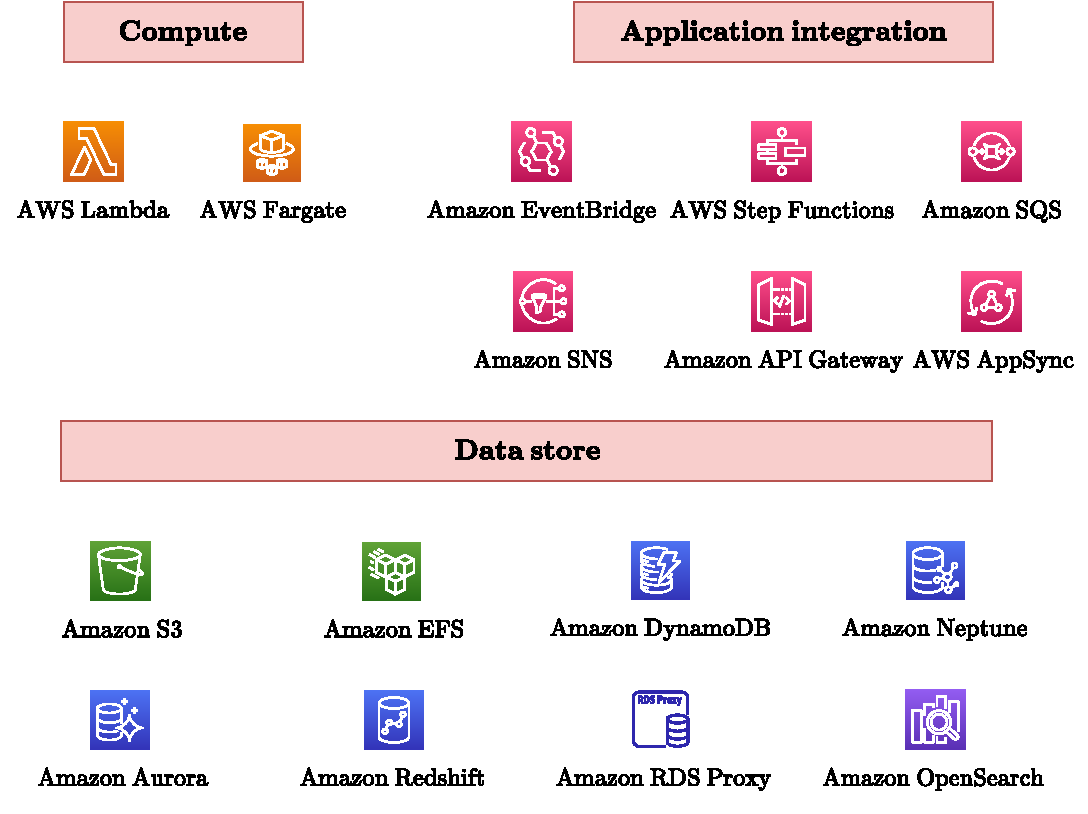
\includegraphics[width=.9\textwidth]{img/AWS-Serverless-1.pdf}
			\caption*{Esempi dei vari servizi \emph{serverless} offerti da Amazon.}
		\end{figure}
	\end{frame}
	
	\section{Architettura FaaS: Microsoft Azure Functions}
	\begin{frame}
		\frametitle{Architettura FaaS: Microsoft Azure Functions}
		\framesubtitle{Introduzione}
		Si presentano vari \emph{designing applications} realizzate con Azure che hanno la caratteristica di essere:
		\begin{itemize}
			\item Scalabili
			\item Sicure
			\item Altamente disponibili
		\end{itemize}
		\begin{figure}
			\centering
			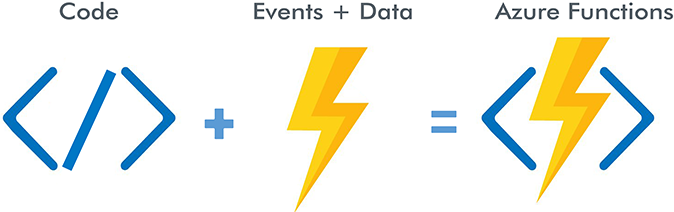
\includegraphics[width=.8\textwidth]{img/azure-functions-cover.png}
		\end{figure}
	\end{frame}
	
	\subsection{Azure Functions in un ambiente ibrido}
	\begin{frame}
		\frametitle{Azure Functions in un ambiente ibrido}
		\begin{figure}
			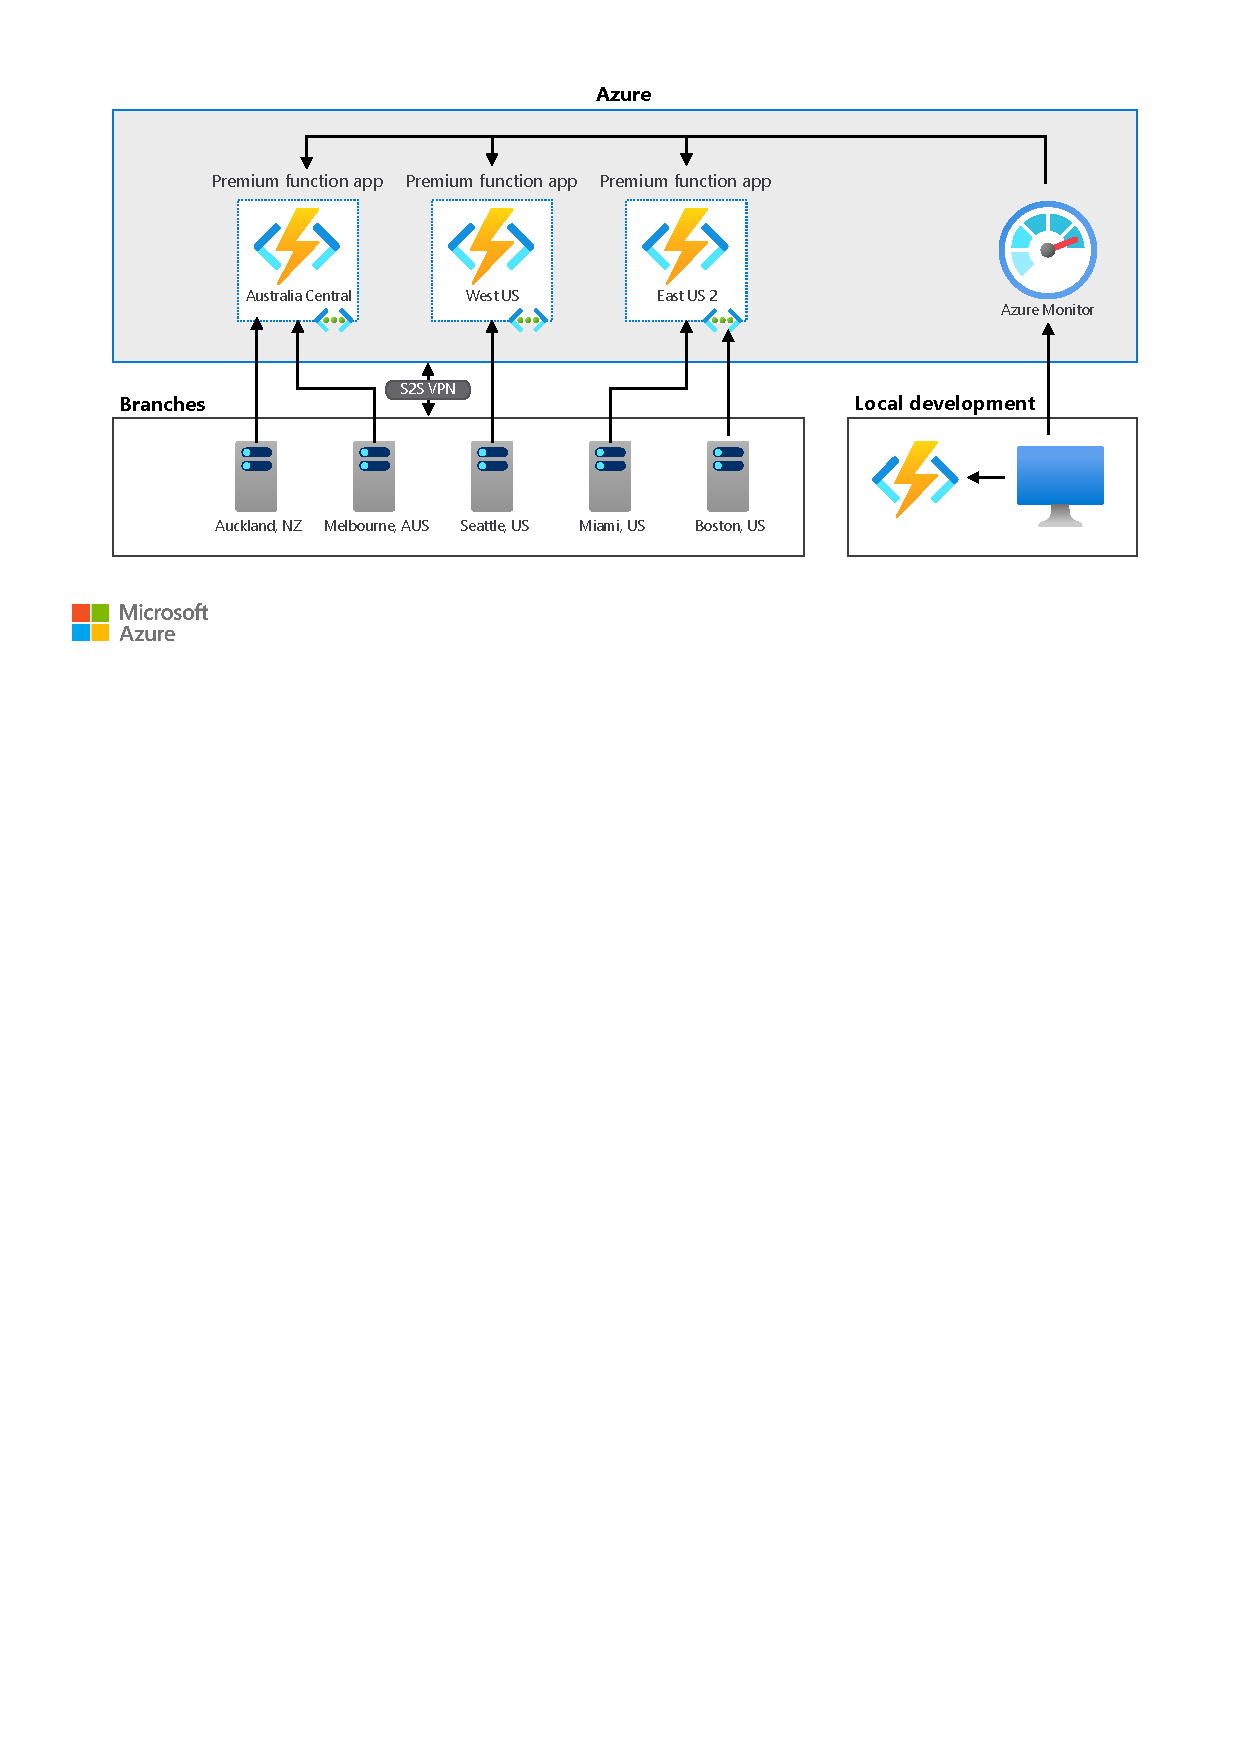
\includegraphics[width=\textwidth]{img/azure-functions-hybrid.pdf}
		\end{figure}
	\end{frame}
	
	\subsection{Automatizzazione cloud \emph{event-based}}
	\begin{frame}
		\frametitle{Automatizzazione cloud \emph{event-based}}
		\begin{figure}
			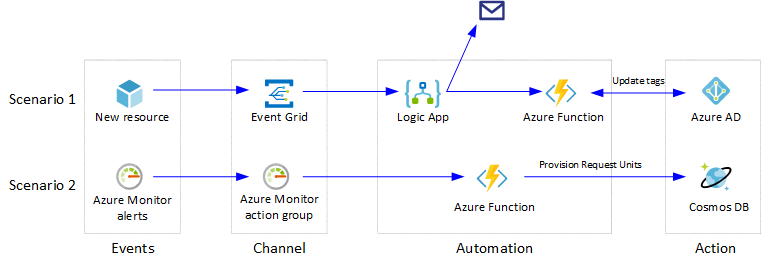
\includegraphics[width=\textwidth]{img/cloud-automation.png}
		\end{figure}
	\end{frame}
	
	\subsection{Soluzioni Multicloud con Framework Serverless}
	\begin{frame}
		\frametitle{Soluzioni Multicloud con Framework Serverless}
		\begin{figure}
			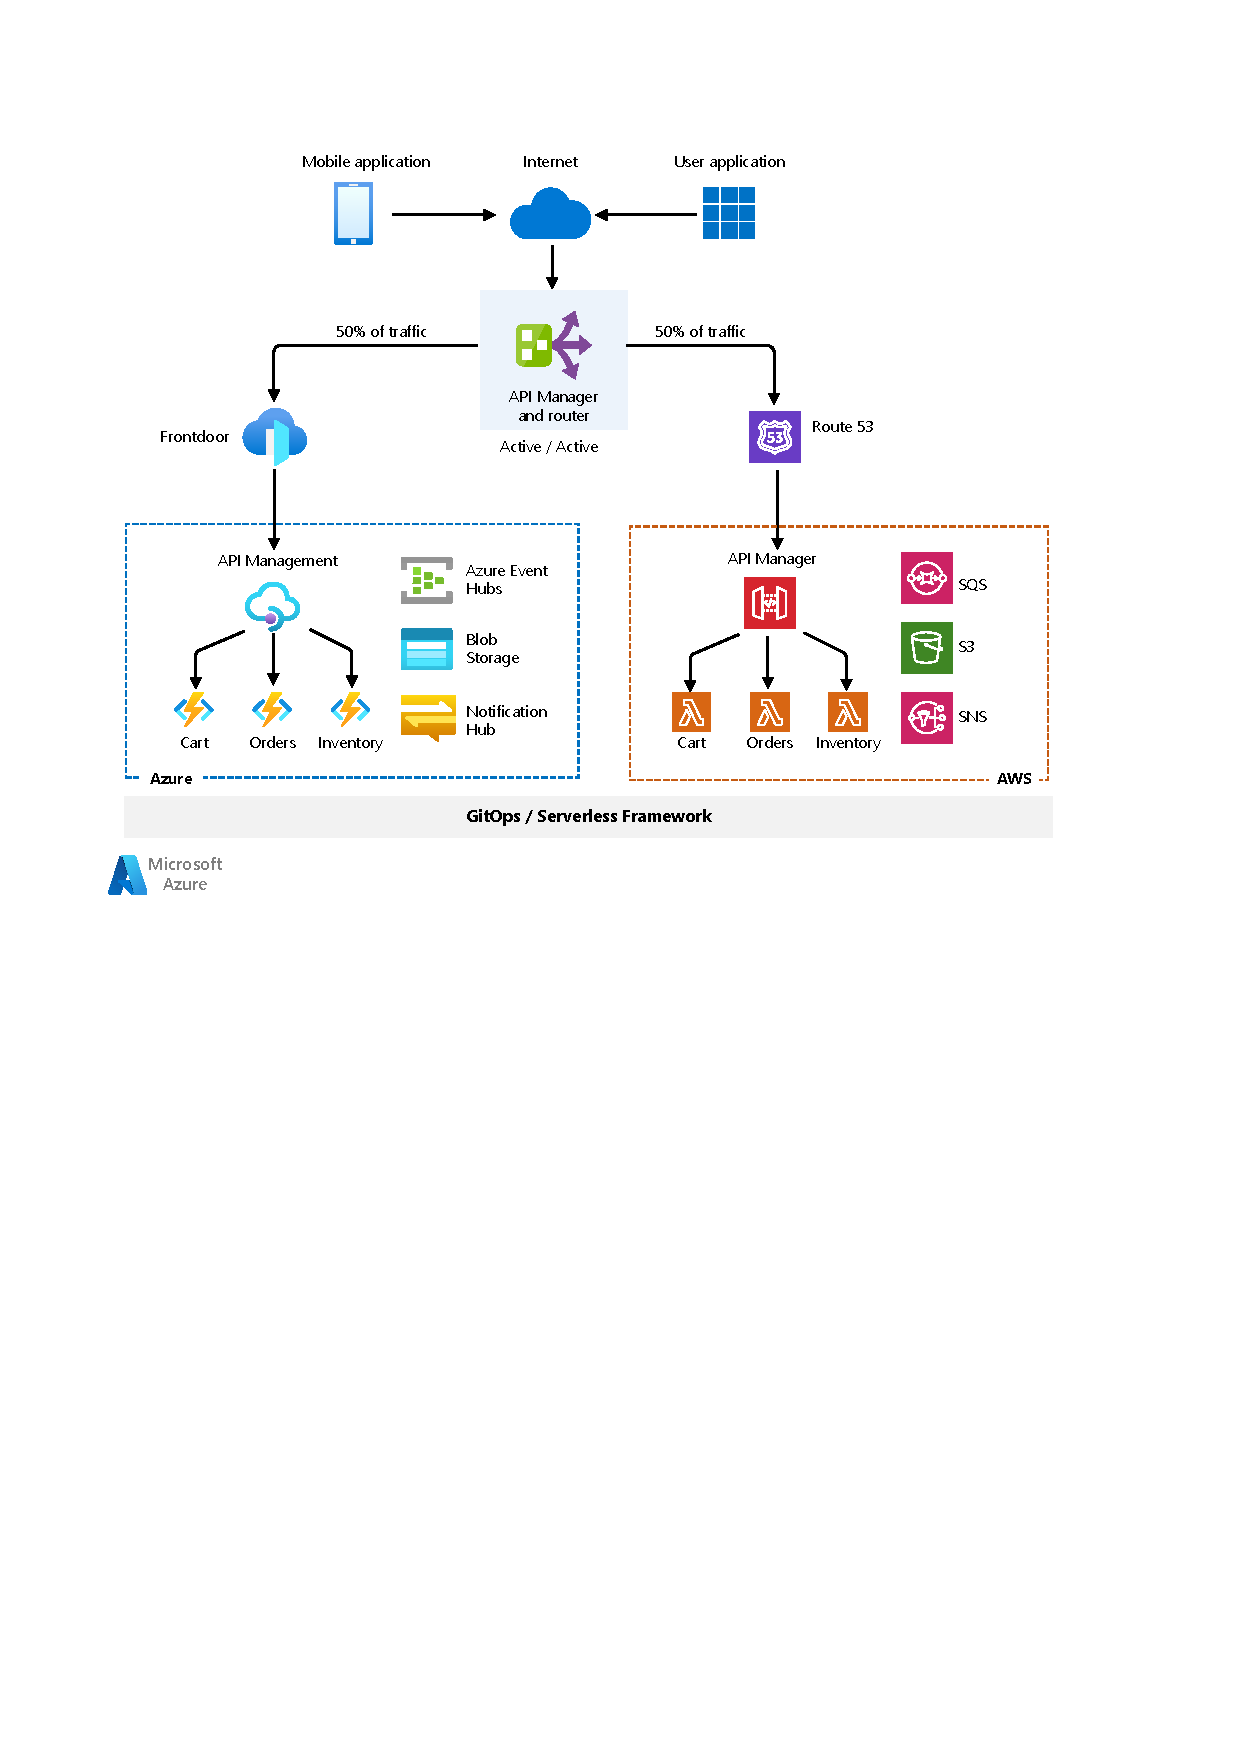
\includegraphics[width=\textwidth]{img/multi-cloud-serverless-architecture.pdf}
		\end{figure}
	\end{frame}
	
	\subsection{Condivisione della posizione in tempo reale}
	\begin{frame}
		\frametitle{Condivisione della posizione in tempo reale}
		\begin{figure}
			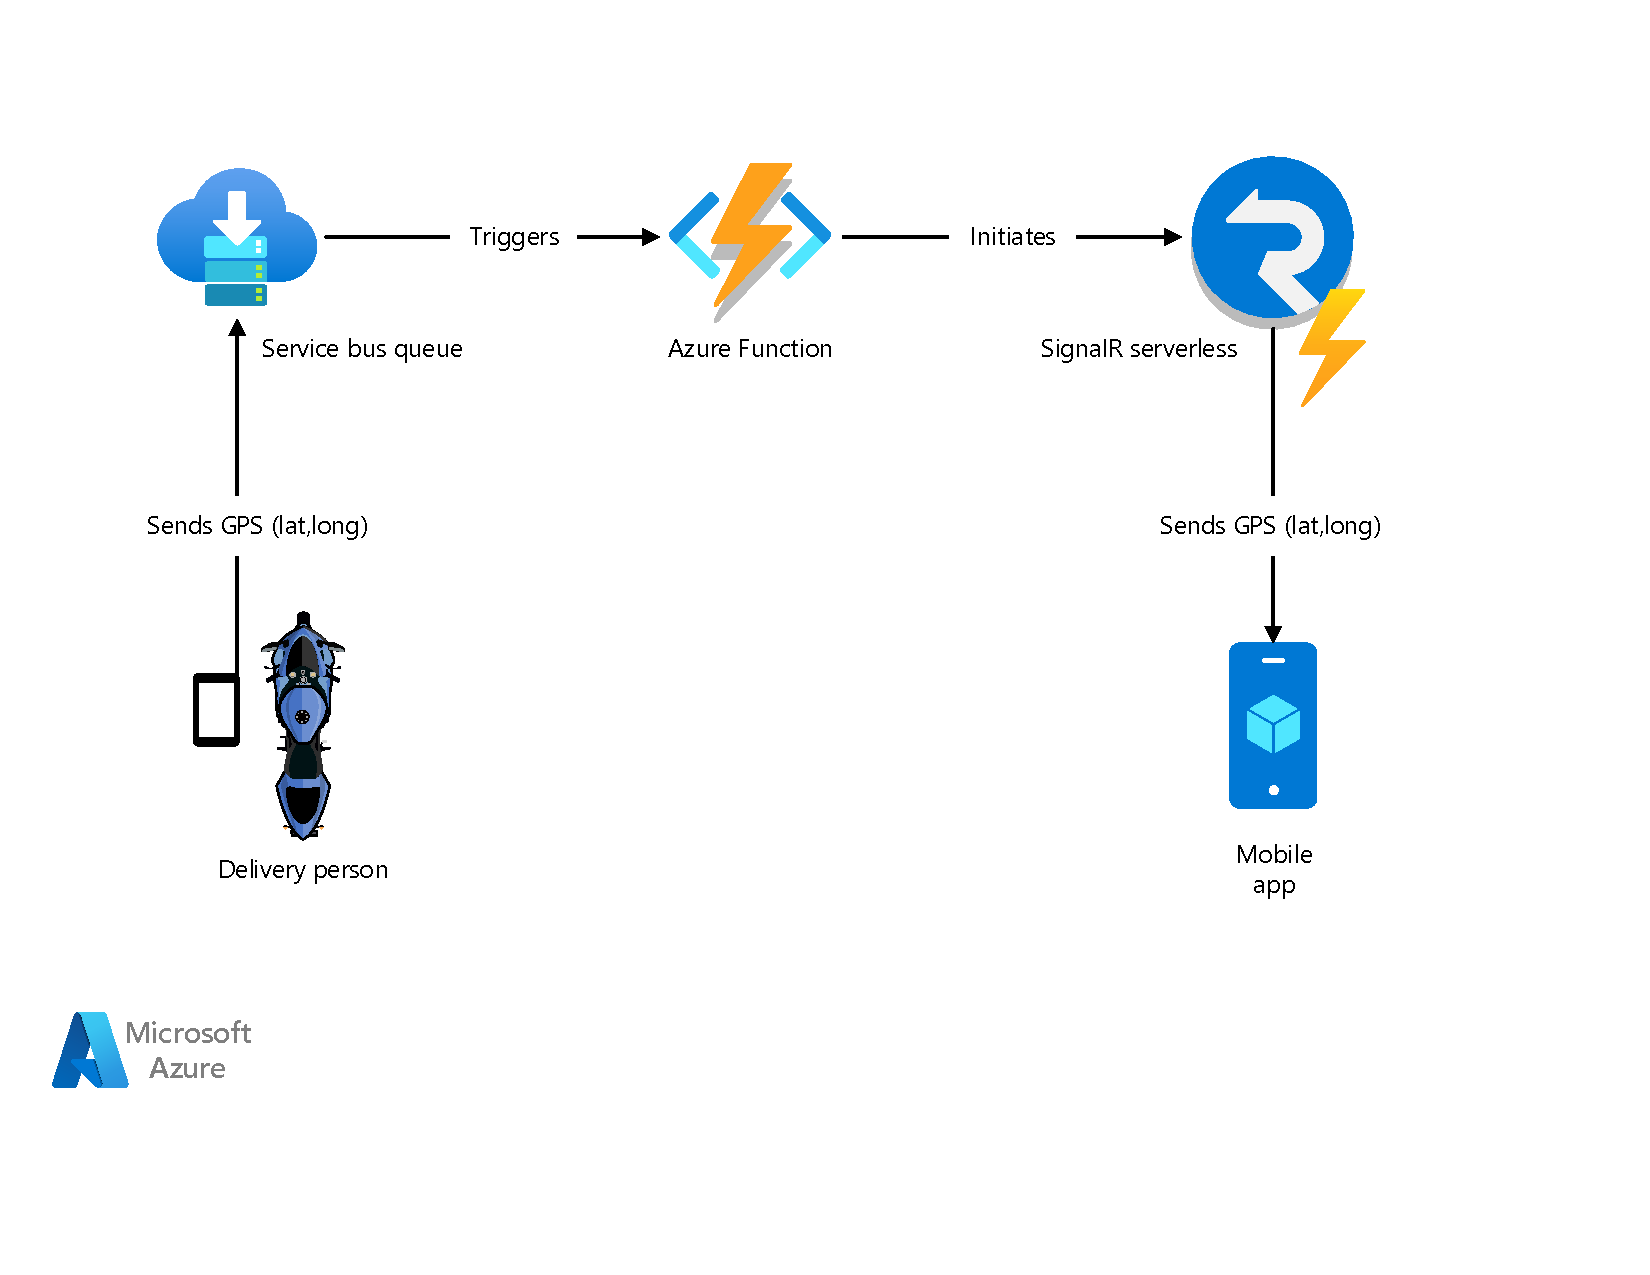
\includegraphics[width=\textwidth]{img/archdiagram.pdf}
		\end{figure}
	\end{frame}
	
	\subsection{Serverless event processing}
	\begin{frame}
		\frametitle{Serverless event processing}
		\begin{figure}
			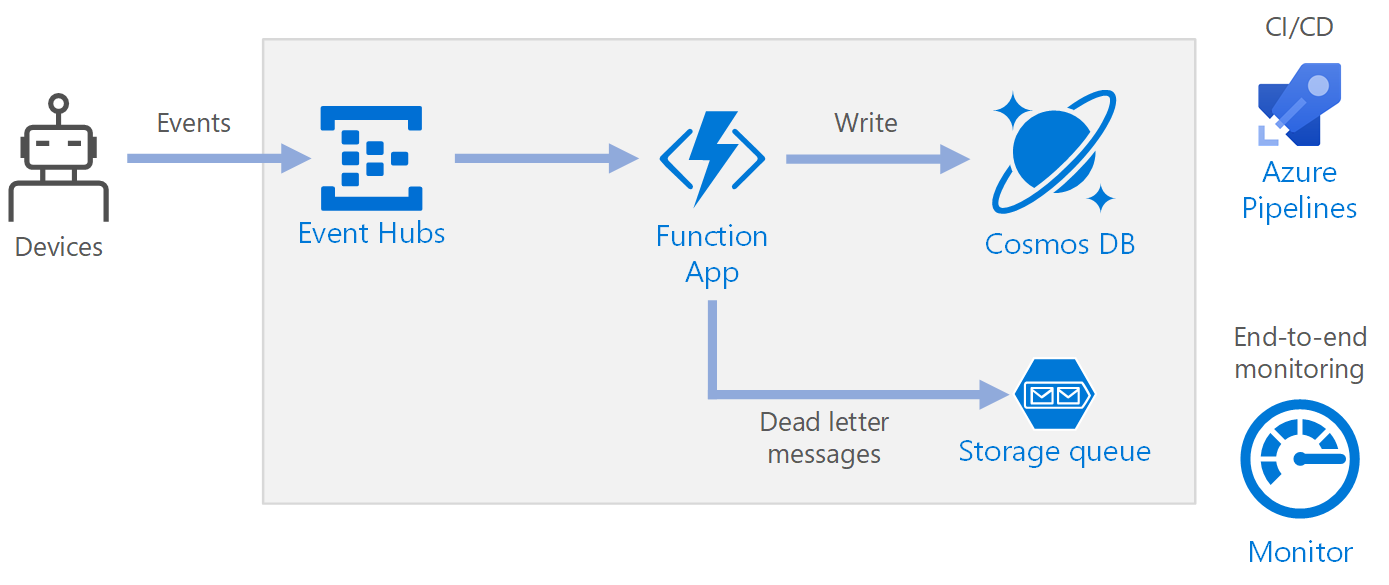
\includegraphics[width=\textwidth]{img/serverless-event-processing.png}
		\end{figure}
	\end{frame}
	
	\section{Esempi di applicazione su Azure}
	\begin{frame}
		\frametitle{Esempi di applicazione su Azure}
		\begin{enumerate}
			\item Sviluppo progetto API in locale;
			
			\item Creazione e sviluppo (\emph{deploy}) delle API create;
			
			\item Tour rapido sulla piattaforma cloud Azure;
			
			\item Test delle API create su un server reale.
		\end{enumerate}
	\end{frame}
	
	\section{References}
	\begin{frame}
		\frametitle{References 1/2}
		\begin{columns}
			\begin{column}{0.5\textwidth}
				\begin{itemize}					
					\item \href{https://www.ibm.com/topics/faas}{IBM - FaaS}
					
					\item \href{https://www.ibm.com/case-studies/greenq-ltd}{IBM - Case study GreenQ}
					
					\item \href{https://www.redhat.com/en/topics/cloud-native-apps/what-is-faas}{RedHat - What is Function-as-a-Service}
					
					\item \href{https://aws.amazon.com/}{AWS Functions}
					
					\item \href{https://cloud.google.com/functions}{Google Cloud Functions}
					
					\item \href{https://azure.microsoft.com/en-gb/resources/cloud-computing-dictionary/what-is-azure/}{Microsoft Azure Cloud}
					
					\item \href{https://www.oracle.com/cloud/}{Oracle Cloud Infrastructure}
					
					\item \href{https://www.ibm.com/topics/serverless}{IBM - What is serverless?}
					
					\item \href{https://aws.amazon.com/serverless/}{Serverless AWS}
				\end{itemize}
			\end{column}
			\begin{column}{0.5\textwidth}
				\begin{itemize}
					\item \href{https://learn.microsoft.com/en-us/azure/architecture/reference-architectures/serverless/event-processing}{Serverless event processing}
					
					\item \href{https://learn.microsoft.com/en-us/azure/architecture/example-scenario/signalr/}{Share a location in real time}
					
					\item \href{https://learn.microsoft.com/en-us/azure/architecture/example-scenario/serverless/serverless-multicloud}{Multicloud solutions (Serverless Framework)}
					
					\item \href{https://learn.microsoft.com/en-us/azure/architecture/reference-architectures/serverless/cloud-automation}{Event-based cloud automation}
					
					\item \href{https://learn.microsoft.com/en-us/azure/architecture/hybrid/azure-functions-hybrid}{Azure Functions in a hybrid environment}
					
					\item \href{https://learn.microsoft.com/en-us/azure/architecture/serverless-quest/serverless-overview}{Serverless functions arch. design}
					
					\item \href{https://aws.amazon.com/solutions/case-studies/coca-cola-freestyle/}{AWS - Case study Coca-Cola}
				\end{itemize}
			\end{column}
		\end{columns}
	\end{frame}
	
	\begin{frame}
		\frametitle{References 2/2}
		\begin{itemize}
			\item \href{https://learn.microsoft.com/en-us/azure/azure-functions/functions-scenarios}{Azure Functions scenarios}
			
			\item \href{https://www.oracle.com/cloud/cloud-native/functions/}{Oracle Cloud Infrastructure (OCI)}
			
			\item \href{https://www.oracle.com/customers/generali/}{OCI - Case study Generali Assicurazioni}
			
			\item \href{https://customers.microsoft.com/en-GB/story/1533527200966057333-fujitsu-azure-partner-professional-services-business-critical}{Azure - Case study Fujitsu}
			
			\item \href{https://cloud.google.com/customers/commerzbankag}{Google - Case study Commerzbank}
		\end{itemize}
	\end{frame}
\end{document}